\documentclass[../../main]{subfiles}
\begin{document}
\chapter{GEAR BOX DESIGN}


The objective of this part of the project was to design a couple of
rugged, efficient, and lightweight middle drive wheels integrated with a
gearbox that can provide the needed torque and speed for the AGV.

\subsection*{Key objectives included:}

\begin{enumerate}
\def\labelenumi{\arabic{enumi}.}
\item
  To design the system in SolidWorks.
\item
  Check for structural integrity at operational loads.
\item
  Analyze gearbox performance for the required torque and speed to
  achieve a gear ratio of 20:1.
\item
  Simplify design for manufacturability and assembly.
\end{enumerate}

\section{Literature Survay}

AGVs are driverless transport systems used in the manufacturing
industry, warehouses, and logistics. According to Groover (2015), in
"Automation, Production Systems, and Computer-Integrated Manufacturing,"
an AGV would have a navigation system, a drive system, and sensors to
operate autonomously. The driving system is the major component of an
AGV, which provides the stability of the robot, the load-carrying
capability, and the accuracy of motion.

In AGVs, middle drive wheels are important for balance and drive.
Jazar\textquotesingle s study, "Vehicle Dynamics: Theory and
Applications", presented in the year 2019, gave much importance to wheel
type, selection of motor, and gearbox that affects energy efficiency in
a robot, how much load a robot can carry, adaptation on various kinds of
terrain. A gearbox allows for the delivered torque and speed to the
wheel for smooth, accurate movement.

Research on gearbox design for robotics has highlighted the requirement
for compact, high-efficiency mechanisms. Kauffenberger et al. (2018)
studied gear mechanisms in small mobile robots and found that among
them, spur gears are the most used due to their simplicity, high load
capacity, and ease of manufacturing. Their study also discussed the
trade-off between gear ratios and torque output, noting that planetary
gear systems provide higher torque.

The design of the drive wheel is critical for traction, maneuverability,
and load-carrying capability. Bloss (2017), in "Mobile Robotics:
Principles and Design," has discussed the role of drive wheels in
robots, and he mentioned that material, tread pattern, and diameter of
the wheel have a direct influence on performance. The wheels for AGVs
are designed to meet both lightweight and high durability to allow for
continuous operation with various loads.

The CAD tools utilized for the design of robot systems are quite
popular, due to their advanced modeling and simulation capabilities. Das
and Jana 2020, in the work "Application of CAD Tools in Robotic Design",
have shown the capability of solid works to model complex assemblies
such as gearboxes and also to simulate their motions.

Material selection is one of the most critical aspects in mechanical
design. Ashby, 2011, "Materials Selection in Mechanical Design"
described a criterion for material selection that was based on strength,
weight, cost and environmental considerations. Since this project dealt
with drive wheels it mostly utilized rubberized materials, hence a thick
rubber material was chosen, while gears are made from hardened steel
preferred for its wear resistance and strength, it was also considered
in my material selection.

\section{ Realistic Constraints}

In designing the two middle drive wheels with a gearbox in CAD,
(SolidWorks), considerations to realistic constraints must be made to
ensure the design is practical, manufacturable, and functional. Many a
time, these constraints are classified into technical, material,
economic, environmental, and human factors.

\subsection{Technical Constraints}

These refer to limitations pertaining to the design\textquotesingle s
feasibility and functionality.

\emph{Dimensional Accuracy:} The dimensions need to be precise so that
the fitted parts inside assemble well.

\emph{ Load Bearing Capacity:} The wheels and gearbox should bear the
expected loads without deforming or failing.

\emph{Speed and Torque Requirements:} The gear ratio and wheel design
must be such that desired performance is achieved.

\emph{Compatibility with Other Components}: Ensure that the design fits
well with the AGV chassis, sensors, and other systems.

\emph{Assembly and Maintenance:} The design must ensure ease assembly,
disassembly, and maintenance.

\emph{Simulation Accuracy:} Limitations of CAD software may affect the
accuracy of stress, motion, or thermal simulations.

\subsection{Material Constraints}

The choice of materials impacts weight, durability, and cost.

\emph{Strength and Durability:} Materials must be able to handle the
mechanical stresses without failure.

\emph{Weight:} Lighter materials are always preferred for efficiency,
but without sacrificing strength.

\emph{Availability}: Materials selected must be available to the
required quantity.

\emph{Cost}: The high-performance material may be beyond the budget and
therefore some compromise may be necessary.

\subsection{Manufacturing Constraints}

The design should consider the limitations of manufacturing methods.

Process Feasibility: The parts must be manufacturable using available
processes such as CNC machining, casting or 3D printing.

\emph{Tool Accessibility:} Shapes that include internal grooves or
undercuts may not easily be machined due to complexity.

\emph{Surface Finish:} Very complicated surfaces may be expensive or
time-consuming to produce.

\emph{Assembly Difficulty:} Designs that include many parts or tight
clearances may be more difficult to assemble because of mating with
specific part which may not be possible if there are too tight.

\emph{Standard Components:} Using off-the-shelf components such as
bearings and shafts rather than customized components simplifies
production and reduces cost.

\subsection{Economic Constraints}

The design should be within the financial scope of the project.

\emph{Material Cost}: High-quality materials can also raise costs.

\emph{Manufacturing Cost:} Complex geometries and tight tolerances raise
production costs.

\emph{Time Constraints:} Designs, prototyping, and testing may be too
time-consuming and hence may require simplifications.

\subsection{Environmental Constraints}

The design must ensure a minimal impact on the environment.

\emph{Energy Efficiency:} The system shall minimize energy losses, for
example, frictional losses or heat dissipation.

\emph{Material Sustainability:} Materials used should be recyclable or
eco-friendly wherever possible.

Waste Management: Waste generated in manufacturing is minimized.

\emph{Operating Environment}: The system should be able to put up with
all forms of environmental conditions, including humidity, dust, or an
extreme temperature.

\subsection{Human Constraints}

The human factors bear on the usability and safety.

\emph{Ergonomics:} The system shall be easy to handle during assembly
and maintenance.

\emph{Safety:} Ensure the design minimizes sharp edges or exposed moving
parts that could cause injury.

\emph{User Expertise}: The design shall take into consideration the
expertise of the operators or assemblers.

\emph{Documentation}: Clear assembly and operating instructions are
essential for effective use.

\section{Methodology}

The methodology followed for the project in brief is given below:

\begin{enumerate}
\def\labelenumi{\arabic{enumi}.}
\item
  Determination of dimensions, number of all gear teeth , and gear
  ratio.
\item
  3D Modeling: Detailed CAD modeling of wheels, gears, shafts, and
  housing on SolidWorks.
\item
  Simulation: motion analysis to validate the design.
\item
  Optimization: Refined design for performance and manufacturability.
\end{enumerate}

\subsection{Dimensions}

Ring gear which is the bigger gear has a dimater of 190 teeth

The planet gear has a diameter of 90mm

The sun gear has a diameter of 10mm
\begin{figure}[h]
  \centering
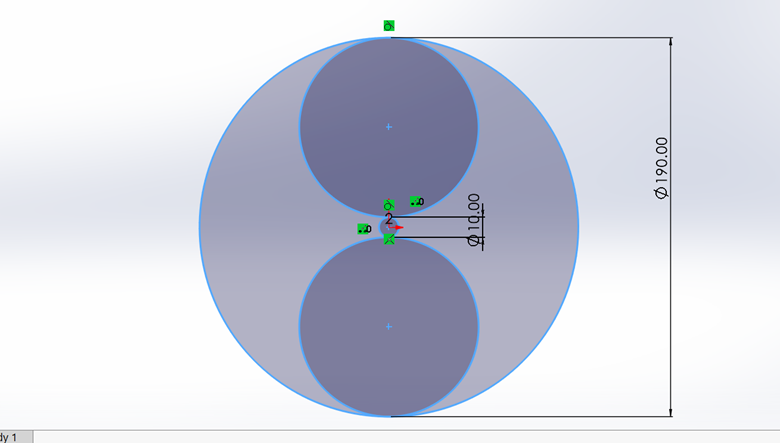
\includegraphics[width=\textwidth]{sublatex/Opryrmi/media/image1.png}
\caption{Add caption here}
\end{figure}

\newpage
\section{3D Modeling}

Following components were modelled using SolidWorks:



  \subsection{Middle Drive Wheels:}
  For Traction and load-carrying capacity. Which is
  made of natural rubber has the ability to withstand high load and
  relatively not so heavy. The wheels for AGVs are designed to meet both
  lightweight and high durability to allow for continuous operation with
  various loads.
  \begin{figure}[h]
    \centering
    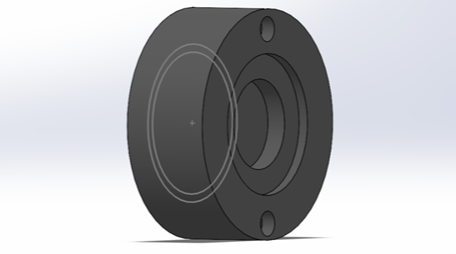
\includegraphics[width=0.8\textwidth]{sublatex/Opryrmi/media/image2.png} 
    \caption{Caption 1}
  \end{figure}


% \begin{figure}[ht]
%   \centering
%     \begin{subfigure}[b]{0.35\textwidth}
%         \centering
%         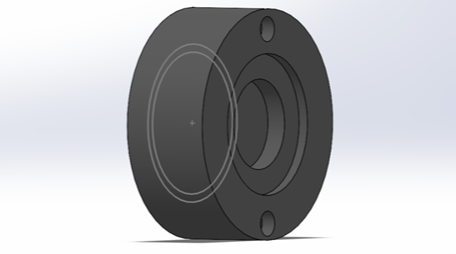
\includegraphics[width=\textwidth]{sublatex/Opryrmi/media/image2.png} 
%         \caption{Caption 1}
%     \end{subfigure}
%     \hspace{1em}
%     \begin{subfigure}[b]{0.45\textwidth}
%         \centering
%         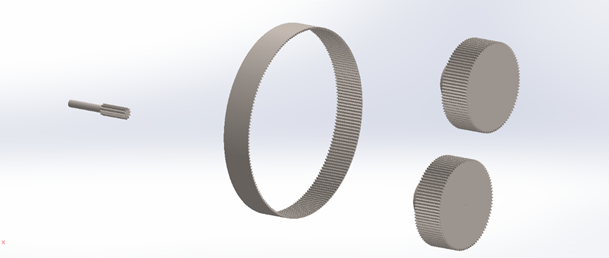
\includegraphics[width=\textwidth]{sublatex/Opryrmi/media/image3.png} 
%         \caption{Caption 2}
%     \end{subfigure}
%     \caption{Main caption for all images}
%     \label{fig:three_images}
% \end{figure}


\subsection{Gearbox:}
Compact design with spur gears for efficient transmission.
Studies shows spur gears are the most used due to their simplicity, high
load capacity, and ease of manufacturing. Their study also discussed the
trade-off between gear ratios and torque output, noting that planetary
gear systems provide higher torque.
\begin{figure}[h]
  \centering
  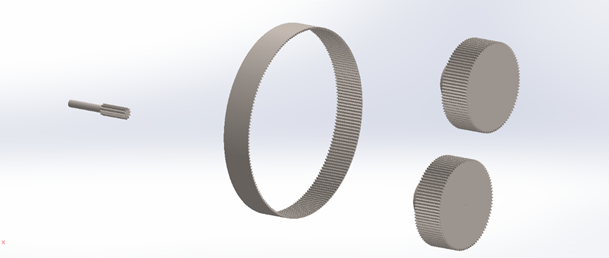
\includegraphics[width=0.8\textwidth]{sublatex/Opryrmi/media/image3.png} 
  \caption{Caption 1}
\end{figure}

\subsection{Shafts and Bearings:} 
For smooth rotation and distribution of loads.
I made use of both skf bearing 108tn92 and skf bearing 1210ektn9202
while for the wheel holder it was made with hard steel for firmness and
durability.
\begin{figure}[h]
  \centering
  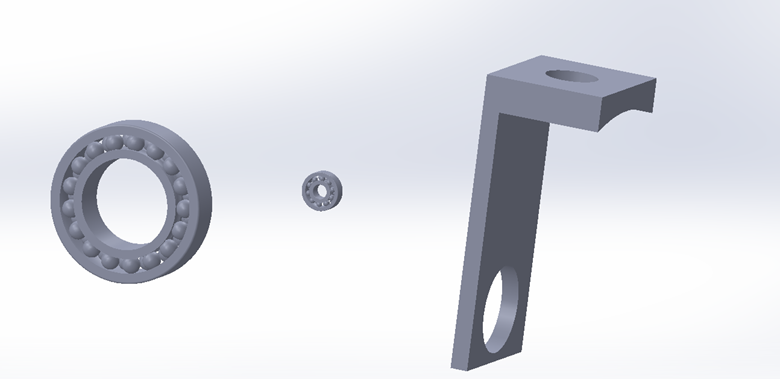
\includegraphics[width=0.8\textwidth]{sublatex/Opryrmi/media/image4.png} 
  \caption{Caption 1}
\end{figure}

\subsection{Housing:} 
Enclosed system for protection against dust and debris.
Which lightweight aluminum were used to reduce the weight of the gear
box.
\begin{figure}[h]
  \centering
  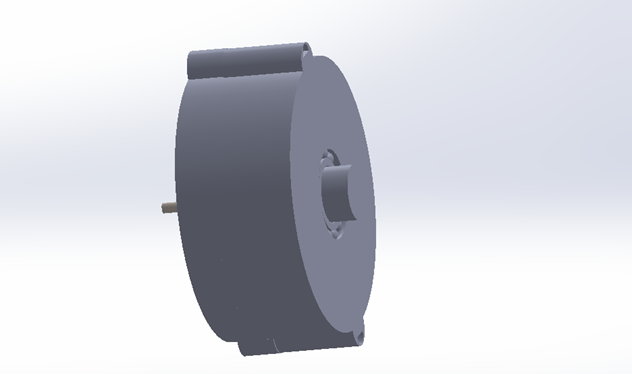
\includegraphics[width=0.8\textwidth]{sublatex/Opryrmi/media/image5.png} 
  \caption{Caption 1}
\end{figure}

% \begin{figure}[ht]
%   \centering
%     \begin{subfigure}[b]{0.35\textwidth}
%         \centering
%         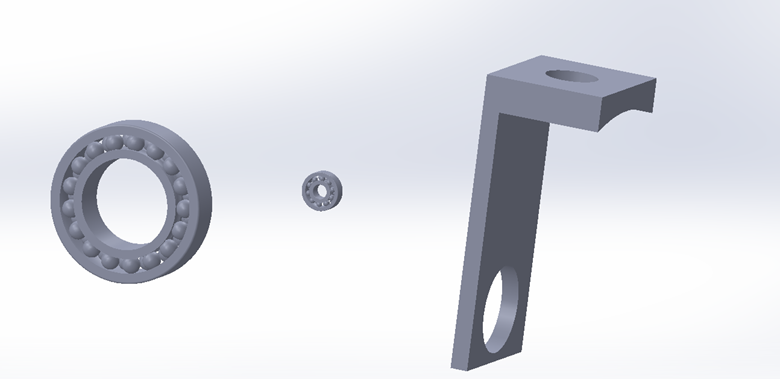
\includegraphics[width=\textwidth]{sublatex/Opryrmi/media/image4.png} 
%         \caption{Caption 1}
%     \end{subfigure}
%     \hspace{1em}
%     \begin{subfigure}[b]{0.45\textwidth}
%         \centering
%         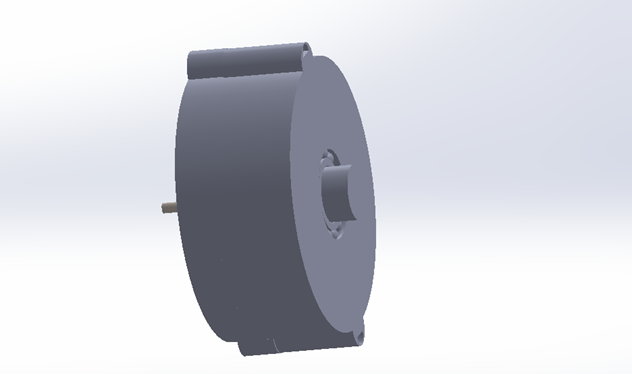
\includegraphics[width=\textwidth]{sublatex/Opryrmi/media/image5.png} 
%         \caption{Caption 2}
%     \end{subfigure}
%     \caption{Main caption for all images}
%     \label{fig:three_images}
% \end{figure}
\newpage
\subsection{Assembly}

The parts were then assembled in SolidWorks for a check on
appropriateness and compatibility.
\begin{figure}[h]
  \centering
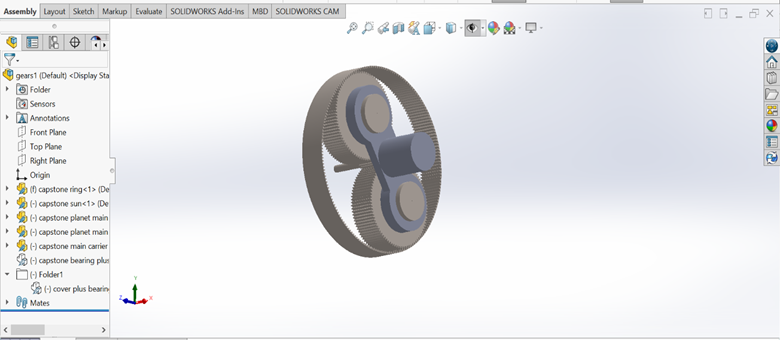
\includegraphics[]{sublatex/Opryrmi/media/image6.png}
\caption{Add caption here}
\end{figure}

\section{Calculation and Analysis}

Simulations done in SolidWorks to test performances of the design:


\subsection{GEARBOX CALCULATION}


\begin{itemize}
\item
  ring gear \(\rightarrow 190\) Teeth {[}120 mm \(\phi\) {]} {[}Tr{]}
\item
  PLAMET Gear \(\rightarrow 90\) Teeth {[}Tp{]}
\item
  Sun gear \(\rightarrow 10\) Teeth {[}Ts{]}
\end{itemize}

GEAR RATIO : NOTE I want a high ratio of $20:1$

\[\begin{aligned}
  20 &= 1 + \cfrac{T_{r}}{T_{s}} \\
  \cfrac{T_{r}}{T_{s}} &= 19 \\
  T_{r} &= 19T_{s}
\end{aligned}\]

The planet does not affect the ratio but determines the spacing of the
sun and ring gears.
Rearanging:

\[\begin{aligned}
\frac{T_{r}}{T_{s}} &= 19 \\
IF\ T_{s} &= 10 \\
T_{r} &= 19*10 = 190
\end{aligned}\]

from \(T_{r} - T_{s} = 2T_{p} \rightarrow\) Spacing in the ring

\[\begin{aligned}
190 - 10 &= 2T_{p} \\
T_{p} &= 90 \\
\ \to 1 + \frac{T_{r}}{T_{s}} &\Rightarrow 1 + \frac{190}{10} = 20 \\
\ \to &20:1
\end{aligned}\]

\(\to 1500\) input speed
\(\div 20(gear\ ratio) \Rightarrow 75rmp\) output speed

Considering\\
Nema 23 stepper motor\\
Nominal power \(\rightarrow 240\) Watts\\
Nominal voltage \(\rightarrow 484\)\\
Nominal current \(\rightarrow 5\text{ }A\)\\
Maminal rotation \(\rightarrow 1500rpm\)

\[T_{\text{in~}} = \frac{P \times 60}{2\pi \times N} = \frac{240 \times 60}{2\pi \times 1500} \Rightarrow T_{\text{in~}} = 1.53Nm\]

\begin{itemize}
\item
  This calalation is assumed \(100\%\) efficiency, Real - Idorly will be
  slightly lower due to losses {[}heat, friction{]}
\end{itemize}

\[\begin{aligned}
T_{\text{out~}}  \  &= T_{\text{in~}} \times R_{\text{atio~}} \times \eta\text{~~} \\
\  &= 1.53 \times 20 \times 0.94 \\
\  &= 28.2Nm
\end{aligned}\]

\[\begin{aligned}
\eta\lbrack\text{~efficiency~}\rbrack = \frac{\text{~Out put power~}}{\text{~Input poise~}} \times 100\% &= \frac{75 \times 28.2}{1500\  \times 1.53} \\
= \frac{2,115}{2,280} &= 0.927 = 92\%
\end{aligned}\]
\newpage


\section{Motion Analysis:}

Wheels\textquotesingle{} rotation and torque transfer in the gearbox
simulated.

Result: Smooth motion with efficiency in power transmission.
\begin{figure}[h]
  \centering
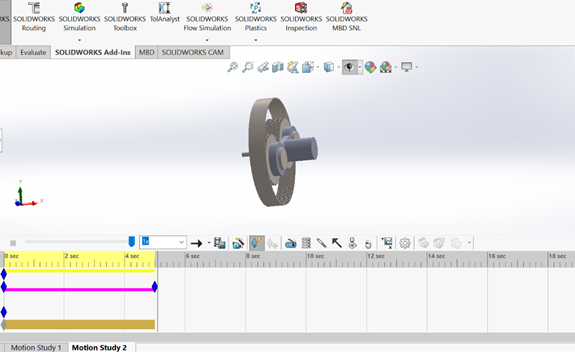
\includegraphics[]{sublatex/Opryrmi/media/image7.png}
\caption{Add caption here}
\end{figure}

\emph{Material Selection}

\emph{Wheels}: Natural rubber, corrosion resistant and high load capacity.

\emph{Gears}: Hardened Steel for increased strength and wear resistance

\emph{Shafts}: Steel for durability

\emph{Housing}: aluminum protection

\emph{Results and Discussion}

The final design was able to meet all the specified requirements, which
included load capacity, torque output, and manufacturability. The
simulations proved that the system was structurally sound and could
operate without hitches under realistic conditions .
\newpage
\section{Conclusion}

It should not only be functional, but also practical, manufacturable,
and economic, taking into consideration all the constraints. The
literature survey focuses on the fact that the gearbox-equipped drive
wheel system is a main concern in the design of an AGV. Material
selection, load-carrying capacity, torque optimization, and
manufacturability are the key factors to be considered. In this paper,
design and simulation for performance improvement of the AGV using
SolidWorks are proposed to overcome these bottlenecks and help in the
development of reliable high-performance drive systems for AGVs.

The middle drive wheels with an integrated gearbox were designed and
further validated for use in an AGV. The system was reliable, efficient,
and easy to manufacture. Future work can be the physical development of
the prototype and performance testing at site applications..


\end{document}